\section{Neural networks}%
\label{sec:Neural networks}

A neural network is a machine learning model, that consists of a set of layers. Neural networks are used to recognize patterns in data and be able to classify it. The way it works is by having some input data that can be used as a input to the network, and then be propageted through each layer. In an untrained network the output would not make much sense, but by training the network with known input and expected output data, a network can give quite accurate results.

\subsection{Fully connected layer}%
\label{sub:Fully connected layer}

The fully connected layer is also known as a dense layer or a linear layer.
The input can be represented as neurons and synapses, with $D$ input neurons and $M$ output neurons. Each input neuron will be connected by synapses to all output neurons.
This layer's input can be represented as a vector $\bm{x}$ and the output can also be represented as a vector $\bm{y}$.
In \autoref{fig:neural_network} it is illustrated what is the input, a connection and the output.

\begin{figure}
    \centering
    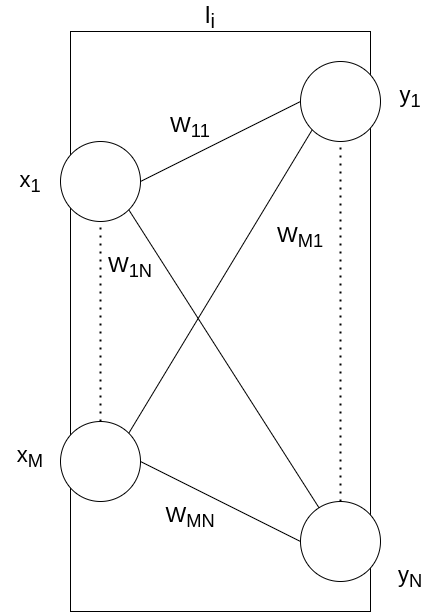
\includegraphics[width=0.5\textwidth]{assets/linear-layer.png}
    \caption{An illustration of a fully connected layer, where the dotted lines means there might be more values in between.}
    \label{fig:neural_network}
\end{figure}


The synapses works by having a weight which is multiplied to the value from the input.
The weights of the synapses can be represented as a matrix $\bm{W}$, which will now be referred to as the weights.
The weight $w_{ij}$ corresponds to the weight between input $i$ and output $j$.
Where $i = 1, ..., D$ and $j = 1, ..., M$.

When data is propagated through this layer, it goes from the input through a synapse, where it is multiplied by the weight and then each value that ends in that output is summed together.

$$y''_j = \sum_{i=0}^D w_{ji}x_i  $$

Once the data has reached the output, there should also be added a bias, which can make the layer be able to fit better to the desired result.
The bias $\bm{b}$ can be represented as a vector with the same length as the output $M$.

$$y'_j = b_j + \sum_{i=0}^D w_{ji}x_i$$

The vector $\bm{y'}$ can thus be represented as a vector to matrix multiplication and adding the bias vector

$$\bm{y'} = \bm{b} + \bm{W}\bm{x}$$

At last there should be applied an activation function, this will be denoted $\sigma$.
So $y_j$ becomes

$$y_j = \sigma \left(y'_j\right)$$

\subsection{Activation functions}%
\label{sub:Activation functions}

Activation functions have an important role in neural networks, since they can introduce non-linearity. This is important when training the network.
Some common activation functions can be seen in \autoref{tab:activation}.

\begin{table}[H]
\centering
\begin{tabular}{|c|c|}\hline
\textbf{Function} & $\bm{\sigma}$ \\\hline
tanh     & $\frac{e^x - e^{-y'}}{e^x + e^{-y'}}$ \\\hline
ReLU     & $max(0, y')$ \\\hline
sigmoid  & $\frac{1}{1+e^{-y'}}$ \\\hline
softmax  & $\frac{e^{y'}}{\sum^K_{k=1} e^{y'_k}}$ \\\hline
\end{tabular}
\caption{A list of common activation functions.}
\label{tab:activation}
\end{table}

\subsection{Convolutional layer}

A neural network with one or more convolutional layers are called a convolutional neural network.
The convolutional layer is often takes a three dimensional input, where the two dimensions can be an image and the third dimension is the channels. The channels of an image is most often the different color channels such as red, green and blue.

The goal of a convolutional layer is to detect certain features, in the given input. The network will be able to detect more and more complex features depending on how many convolutional layers the network has.

The convolutional layer works by having a kernel $\bm{K}$ that convolves through the input. The kernel should not be confused with kernels in cuda, it is also known as a filter. The kernel has the same number of dimensions as the input, but the sizes of the image dimensions of the kernel should be less than or equal to the image dimensions of the input. This can be seen on \autoref{fig:conv_input_and_kernel}.

\begin{figure}
    \centering
    \hfill
    \subfloat[][An example for a $3 \times 3$ input to a convolutional layer]{$\begin{bmatrix}
        X_{11} & X_{12} & X_{13} \\
        X_{21} & X_{22} & X_{23} \\
        X_{31} & X_{32} & X_{33} 
    \end{bmatrix}$}
    \hfill
    \subfloat[][An example for a $2\times 2$ kernel]{$\begin{bmatrix}
        K_{11} & K_{12} \\
        K_{21} & K_{22}
    \end{bmatrix}$}
    \hfill
    \null
    \caption{An example for an input and a kernel to be used in a convolutional layer}
    \label{fig:conv_input_and_kernel}
\end{figure}


The convolutional operation works by taking the dotproduct of the kernel with a slice of the input, then adding a bias and applying the activation function. This is done for each channel with the same slice. These values are then stored in the output. This is repeated for a new slice until the the end of the input. The operaion is visualized in \autoref{fig:conv_operation}, the result will be $\bm{Y}''$, to get $\bm{Y}$ there needs to be added a bias and used an activation function.

\begin{figure}
    \centering
    $$\begin{bmatrix}
        \color{red} X_{11} & \color{red} X_{12} & X_{13} \\
        \color{red} X_{21} & \color{red} X_{22} & X_{23} \\
        X_{31} & X_{32} & X_{33} 
    \end{bmatrix} \otimes K \Rightarrow \begin{bmatrix}
        \color{red} X_{11} K_{11} + X_{12} K_{12} + X_{21} K_{21} + X_{22} K_{22} & \\
         &
    \end{bmatrix}$$\\
    $$\begin{bmatrix}
        X_{11} & \color{red} X_{12} & \color{red} X_{13} \\
        X_{21} & \color{red} X_{22} & \color{red} X_{23} \\
        X_{31} & X_{32} & X_{33} 
    \end{bmatrix} \otimes K \Rightarrow \begin{bmatrix}
         Y''_{11} &\color{red} X_{12} K_{12} + X_{13} K_{13} + X_{22} K_{22} + X_{23} K_{23} \\
         &
    \end{bmatrix}$$\\
    $$\begin{bmatrix}
        X_{11} & X_{12} & X_{13} \\
        \color{red} X_{21} & \color{red} X_{22} & X_{23} \\
        \color{red} X_{31} & \color{red} X_{32} & X_{33}
    \end{bmatrix} \otimes K \Rightarrow \begin{bmatrix}
        Y''_{11} & Y''_{12} \\
        \color{red} X_{21} K_{21} + X_{22} K_{22} + X_{31} K_{31} + X_{32} K_{32} & 
    \end{bmatrix}$$\\
    $$\begin{bmatrix}
        X_{11} & X_{12} & X_{13} \\
        X_{21} & \color{red} X_{22} & \color{red} X_{23} \\
        X_{31} & \color{red} X_{32} & \color{red} X_{33}
    \end{bmatrix} \otimes K \Rightarrow \begin{bmatrix}
         Y''_{11} & Y''_{12} \\
         Y''_{21} & \color{red} X_{22} K_{22} + X_{23} K_{23} + X_{32} K_{32} + X_{33} K_{33}
    \end{bmatrix}$$\\
    \caption{A visualization of the convolutional layer operation. The red numbers on the left are the input values that are currently in the window. The red number on the right is the result of the dotproduct of the window and the kernel.}
    \label{fig:conv_operation}
\end{figure}

To put it as a formula for the 2 dimensional image,
let $\bm{X}$ be the input,
$\bm{Y}$ be the output.
$\bm{b}$ be a vector of the bias with the length equal to the number of output channels.
$C_{in}$ the number of input channels.
$\bm{K}$ the kernel.
$k_x$ and $k_y$ the size of the kernel and $s_x$ and $s_y$ be the stride which the kernel is moving through the image.

$$Y_{ijc_{out_l}} = b_{c_{out_l}} + \sum^{C_{in}}_{c = 1} \sum^{i \cdot s_x + k_x}_{i_2 = i \cdot s_x} \sum^{j \cdot s_y + k_y}_{j_2 = j \cdot s_y} X_{i_2j_2c} K_{i_2j_2c} $$

Where $i$ is the index in the first image dimension, $j$ is the index in the second image dimension and $c_{out_l}$ is the current output chnanel.

$i$, $j$ and $l$ are in the following ranges

$$i = 1, ..., \frac{n_x - k_x}{s_x} + 1$$
$$j = 1, ..., \frac{n_y - k_y}{s_y} + 1$$
$$l = 1, ..., C_{out}$$

Where $n_x$ and $n_y$ are the image dimensions.

This means the dimensions of $\bm{Y}$ is

$$\left(C_{out}\right) \times \left(\frac{n_x - k_x}{s_x} + 1\right) \times \left(\frac{n_y - k_y}{s_y} + 1\right) $$

\subsection{Maxpooling layer}

The max pooling layer splits the input into different windows, and outputs the maximum value in each window. The operation is more easily understood in \autoref{fig:max_pool}.

\begin{figure}[htpb]
    \centering
    $$\begin{bmatrix}
        \color{red}1 & \color{red} 2 & \color{green} 3 & \color{green} 4 \\
        \color{red}8 & \color{red}9 & \color{green}10 & \color{green}11 \\
        \color{blue}7 & \color{blue}1 & \color{magenta}2 & \color{magenta}6 \\
        \color{blue}2 & \color{blue}1 & \color{magenta}9 & \color{magenta}3
        \end{bmatrix} \Rightarrow \begin{bmatrix}
        \color{red}9 & \color{green}11 \\
        \color{blue}7 & \color{magenta}9
        \end{bmatrix}$$
    \caption{Illustration of a max pooling operation on a $4\times 4$ matrix with a $2\times 2$ window. The window will process the numbers of the same color and output the same color.}
    \label{fig:max_pool}
\end{figure}

In this example the first slice will be $[1, 2, 8, 9]$, the slice is flattened for easier readability. Then the greatest number is $9$ which will be set in the output. This is repeated for the next slice and then repeated until the window reaches the end of the input.

The maxpooling layer reduces the input, such that only the most important features are carried over to the next layer and thus reducing the number of operaitons needed for the nect layer.

\subsection{Composition of layers}%
\label{sub:Composition}

A neural network does often not accomplish much with a single layer, that means the network should be a composition of layers. A simple neural network with multiple layers is a multilayer perceptron which is a network with only fully connected layers, this can be seen on \autoref{fig:multilayer_perceptron}.

\begin{figure}
    \centering
    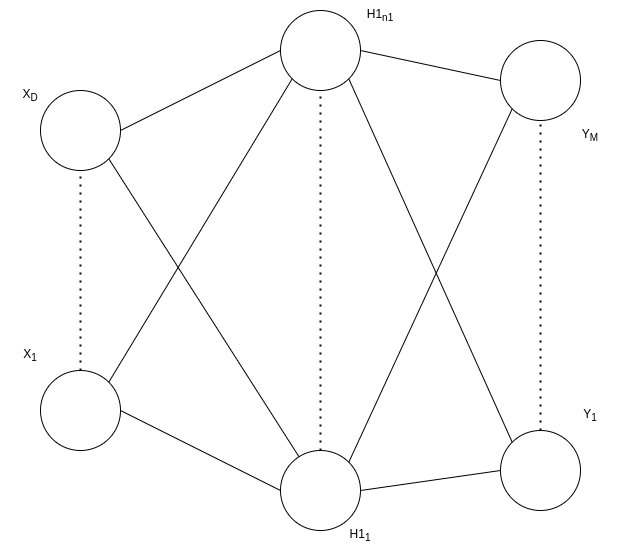
\includegraphics[width=0.6\textwidth]{assets/multilayer-perceptron.png}
    \caption{A multilayer perceptron (a neural network with only fully connected layers). Where $H1_1, ..., H1_{n1}$ are the outputs of the first layer.}
    \label{fig:multilayer_perceptron}
\end{figure}

But the network can be composed how the user likes it, the only restriction is that the number of outputs in one layer has to match with the number of inputs in the next layer. The input for a layer might also need to be transformed from its original shape to the input shape of the next layer.

When composing the layers, the forward propagation function also changes, where the input type will not change, but the output type will be the type of the last layer.
The new forward propagation function will be the following $g_{nnl}$

$$f_{nnl} = f_l(f_{nn})$$

Where $f_l$ is the forward propagation of the layer and $f_{nn}$

\subsection{Loss functions}%
\label{sub:Loss functions}

To determine how close the network is at predicting something, a loss function can be used.
The loss function works by taking the output of the network and comparing it with the expected value or label.
This will be relevant in the following subsection (\autoref{sub:network_training}).

There are different loss functions that finds the loss in different ways. Some common loss functions can be seen in \autoref{tab:loss}

\begin{table}[ht]
\centering
\begin{tabular}{|c|c|}
\hline
\textbf{Loss function}  & \textbf{L(W)} \\ \hline
Cross entropy  & $-\sum^K_{k=1}(l_k\ ln\ y_k)$ \\ \hline
Mean squared error & $\frac{1}{K}\sum^K_{k=1}(y_k-l_k)^2$ \\ \hline
\end{tabular}
\caption{Some common loss functions, where $\bm{y}$ is the output of the network and $\bm{l}$ is the expected values or labels}
\label{tab:loss}
\end{table}

\subsection{Network training}%
\label{sub:network_training}

The goal of using a neural network is to make it correctly classify some input data. This can be done by training the network.
The network can be trained by "optimizing" the weights for each layer. Here optimizing is referred to as giving a better result and not as code optimizing.
One method of optimizing the network is by using gradient descent.
The function $E$ which the gradient will be found, is the forward propagation of the network as a function of the weights, composed with a loss function, which is shown in the following formula.

$$E(\bm{W}) = L(f(\bm{W}_1, \bm{W}_2, ..., \bm{W}_n))$$

Where $n$ is the number of layers in the network, $\bm{W}_i$ is the weights for layer $i$ where $i = 1...n$, $L$ is a loss function and $f$ is the forward propagation.
Gradient descent works because the loss function will be minimized, thus the weights need to change to fit the input and label data.

In \autoref{sec:autodiff} it will be discussed how to find the gradient or derivative of any function, which can be used for gradient descent.

\subsection{Exploding and vanishing gradients problem}

When using the backpropagation algorithm in a neural network, the gradient in some layers might be so small, that when updating the weights of the early layers, they will barely change. This problem is referred to as the vanishing gradients problem, as the gradients become so small that they almost vanish.
This problem makes it much harder to train a network since the weights might never reach the optimal value.
On the other hand the gradients might get so large that they move the weights way too much, such that the weights will never really hit an optimal value.
This problem can make the network significantly harder to train and maybe even impossible. This can, for example, make the application of vanilla SGD impossible \cite{exploding_gradients}.

This problem can be dealt with by using normalization layers which will be discussed in \autoref{sub:norm_layers}.


% There is no well-accepted metric for determining the presence of pathological exploding gradients \cite{exploding_gradients}.

\subsection{Normalizations layers}%
\label{sub:norm_layers}


\subsection{Residual network (ResNet)}

Deep convolutional neural networks have led to a series of breakthroughs for image classification \cite{resnet}.
To solve more and more complex tasks, deeper networks seems to be more accurate.
The problem is that the networks can not just get deeper and deeper since it seems that when a certain limit is reached accuracy is becoming saturated and after adding more layers accuracy seems to degrade.
An obstacle to this problem has also been the problem of vanishing/exploding gradients.
However ResNet is able to be accurate in considerably increased depth and have dealt with the problem of exploding/vanishing gradients by using normalization layers. ResNet also produces results substantially better than previous networks \cite{resnet}.

In this section there will be described which methods ResNet uses and how the model is structured.

% \subsubsection{Residual representation}

\subsubsection{Shortcut connections}

A shortcut connection is a connection that skips one or more layers and may have parameters that change the values.
\autoref{fig:shortcut_connection} shows an example of a shortcut connection that adds the input $\bm{x}$ value of the first layer to the output of the last layer.
Where $F(\bm{x})$ is the forward propagation of the block. The block in this case is just the two weight layers, but in general a block can have any number of layers.
In this case the shortcut connection is an identity mapping, meaning that the connection does not change the value of $\bm{x}$ during the shortcut connection.

\begin{figure}
    \centering
    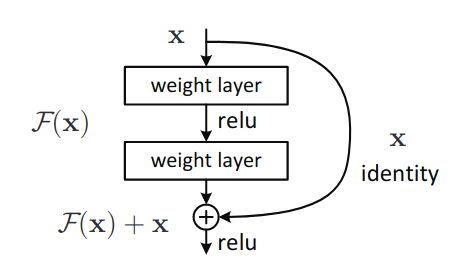
\includegraphics[width=0.55\textwidth]{assets/shortcut-connection.png}
    \caption{A shortcut connection represented by the arching arrow. $\mathcal{F}(\bm{x})$ is the function of applying $\bm{x}$ to the two layers. $\mathcal{F}(\bm{x}) + \bm{x}$ is the value after the shortcut connection. Source: \cite{resnet}}
    \label{fig:shortcut_connection}
\end{figure}

The benefit a shortcut connection is that it deals with the exploding/vanishing gradients problem, since it can allow the gradient to "flow" through to earlier layers, without exploding or vanishing in the same way.

\subsubsection{Deep residual learning}

Residual learning builds on the use of shortcut connections. 
This is done by having shortcuts with identity mapping for every few layers.
The shortcut connections in Eqn.(1) introduce neither extra parameter nor computation complexity \cite{resnet}.
The only extra number of computation that is needed during residual learning is making an element-wise matrix-matrix addition, for every few layers.
The element-wise addition is computationally cheap, thus it can be a very good trade off if it means that the network might be trained faster and it might have better accuracy.

The dimensions of $\bm{x}$ and $\mathcal{F}(\bm{x})$ has to be equal, if they are not the data can be linearly projected by a matrix $\bm{W}_s$ to match the dimensions of $\bm{y} = \mathcal{F}(\bm{x}) + \bm{W}_s\bm{x}$.

\subsubsection{Netwok architecture}%

\autoref{fig:resnet} shows the two network archtectures: plain and residual.

\textbf{Plain network}: The convolutional layers mostly have $3 \times 3$ filters and follow two simple design rules:
(i) for the same output
feature map size, the layers have the same number of filters; and
(ii) if the feature map size is halved, the number of filters is doubled so as to preserve the time complexity per layer
\cite{resnet}.
Whenever the data nis downsampled it is done by a convolutional layer with a stride of 2.
In the end the network has a fully connected layer with 1000 outputs.

\textbf{Residual network}: 
The residual network is based on the plain network, but uses shortcut connctions with identity mapping. However when the dimensions do not match for a shortcut connection (dotted line), the data is downsampled by using a $1 \times 1$ convolution with a stride of 2.

\begin{figure}
    \centering
    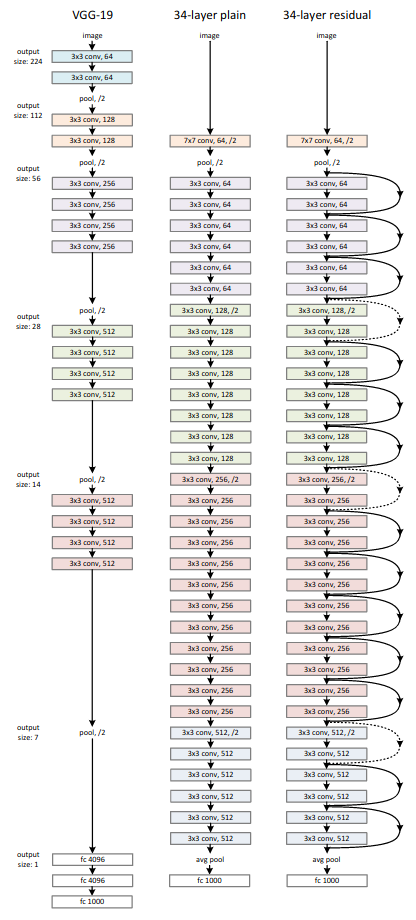
\includegraphics[scale=0.69]{assets/residual-net.png}
    \caption{The first part of each layer tells which type of layer it is, the second tells how many channels the layer uses, and the third tells if there is downsampling ($/2$). \textbf{middle}: 34-layer plain network. \textbf{right}: 34-layer residual network - based on plain, but with shortcut connections. The dotted lines represent a downsampling in the shortcut connection. Source: \cite{resnet}}
    \label{fig:resnet}
\end{figure}


